\section{Intégration et test}

Après la simulation, le chenillard a été intégré depuis le menu FPGA de Logisim, avec la carte \og MAX\_V\_CONSOLE \fg{} comme cible, dans la CPLD MAX V de la carte MAX\_V\_80P\_25P. Le circuit de plus haut niveau utilisé pour l'intégration est \texttt{main}, fourni dans le projet. Il contient le circuit \texttt{chenillard} et relie ses entrées et sa sortie aux boutons, aux interrupteurs, aux LEDs et à l'horloge de la console.

\subsection{Synthèse et vérification du circuit}

L'intégration est lancée depuis la fenêtre Synthesize \& Download (voir \emph{\underline{Figure~\ref{fig:integration_execute}}}). Le circuit \texttt{main} est choisi comme circuit de plus haut niveau (\textit{Toplevel}), la carte \og MAX\_V\_CONSOLE \fg{} comme carte cible et l'action \og Synthesize \& Download \fg{} comme méthode, puis l'exécution est démarrée avec le bouton Execute.

\begin{figure}[H]
	\centering
	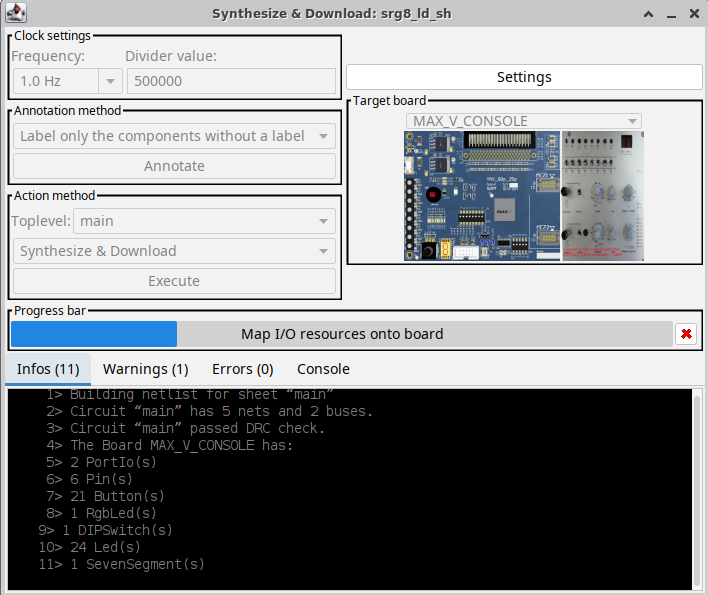
\includegraphics[width=0.6\textwidth]{./images/integration-execute.png}
	\caption{Partie 3, lancement de la synthèse depuis la fenêtre Synthesize \& Download}
	\label{fig:integration_execute}
\end{figure}

Logisim construit d'abord la netlist du circuit \texttt{main}, puis effectue un contrôle des règles de conception (DRC). Les messages de l'onglet Infos montrent que le circuit \og passed DRC check \fg{} et l'onglet Errors n'indique aucune erreur : le circuit est donc valide et peut être synthétisé. Logisim liste ensuite les ressources disponibles sur la carte (boutons, interrupteurs, LEDs, \ldots) et passe à l'étape d'assignation des entrées et sorties, visible dans la barre de progression (\og Map I/O resources onto board \fg{}).

\subsection{Assignation des broches}

Avant la compilation, chaque composant d'entrée et de sortie du circuit \texttt{main} doit être associé à une ressource physique de la carte, selon l'assignation imposée par la donnée du laboratoire :
\begin{itemize}
	\item les commandes \texttt{load\_i}, \texttt{enable\_i} et \texttt{right\_nLeft\_i} sont reliées aux boutons LOAD, EN et R\_nL de la carte MAX V ;
	\item le pattern \texttt{pattern\_i} est réglé avec les 8 interrupteurs S0 à S7 de la console ;
	\item la sortie \texttt{led\_o} est affichée sur les 8 LEDs L0 à L7 de la console ;
	\item l'horloge \texttt{clk\_i} est connectée au signal d'horloge de la console (pin 27a).
\end{itemize}

L'assignation se fait dans la fenêtre Component to FPGA board mapping (voir \emph{\underline{Figure~\ref{fig:integration_mappage}}}) en sélectionnant chaque composant puis la ressource correspondante sur l'image de la carte. Une fois l'assignation terminée, la liste Unmapped Components est vide et tous les composants (\texttt{clk\_i}, \texttt{enable\_i}, \texttt{LED\_0} à \texttt{LED\_7}, \ldots) apparaissent dans la liste Mapped Components. Tous les signaux du circuit sont alors reliés à une ressource de la carte et l'assignation est validée avec le bouton Done.

\begin{figure}[H]
	\centering
	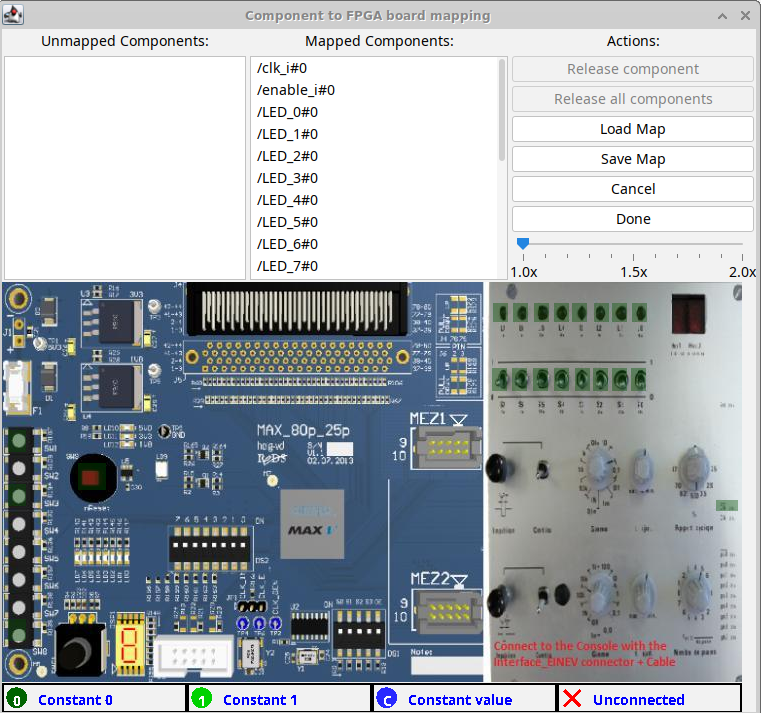
\includegraphics[width=0.6\textwidth]{./images/integration-mappage.png}
	\caption{Partie 3, assignation terminée, tous les composants sont reliés à la carte}
	\label{fig:integration_mappage}
\end{figure}

\subsection{Compilation et programmation}

Une fois l'assignation validée, Logisim génère la description VHDL du circuit, puis Quartus la compile et programme la CPLD de la carte MAX\_V\_80P\_25P par le câble USB-Blaster. La programmation s'est terminée sans erreur et la carte a pu être testée.

\subsection{Test sur la carte}

Une fois la carte programmée, le chenillard a été testé sur le matériel réel. La boîte de commande est connectée au connecteur SUBD25 de la carte MAX V et génère l'horloge du système, réglée à une fréquence de 1 à 4~Hz afin que la rotation du pattern soit visible à l'\oe il nu sur les LEDs. Une LED allumée correspond à un bit à 1. Le montage utilisé est présenté à la \emph{\underline{Figure~\ref{fig:integration_montage}}}.

\begin{figure}[H]
	\centering
	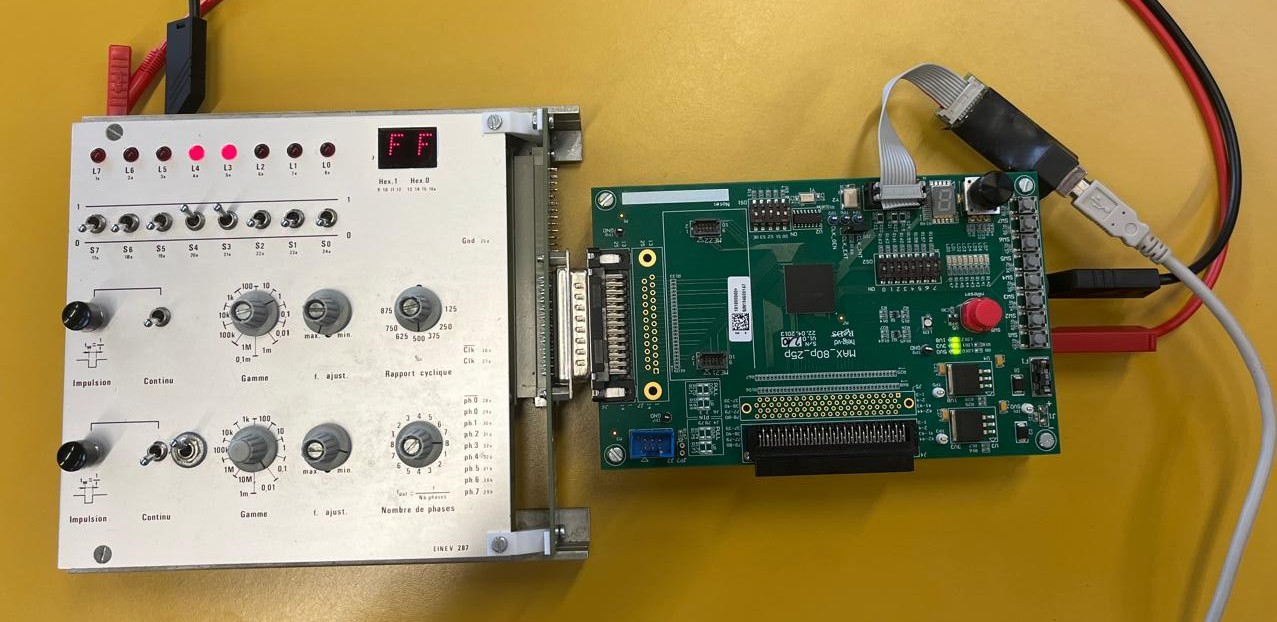
\includegraphics[width=0.6\textwidth]{./images/integration-montage.jpeg}
	\caption{Partie 3, montage de la carte MAX V reliée à la console}
	\label{fig:integration_montage}
\end{figure}

Sur cette photo, la carte MAX V (en bas) est alimentée et programmée par le câble USB-Blaster, et reliée à la console (en haut) par le connecteur SUBD25. Les LEDs L4 et L3 de la console sont allumées, ce qui correspond au pattern \texttt{0001 1000} chargé dans le chenillard, le même que celui utilisé en simulation (voir \emph{\underline{Chronogramme~\ref{fig:simu_p3}}}).

Les tests reprennent chacune des fonctions du chenillard : le chargement d'un pattern avec le bouton LOAD, la rotation à droite et la rotation à gauche avec le bouton EN et le choix du sens avec le bouton R\_nL, l'arrêt de la rotation lorsque EN est relâché, ainsi que le reset. Les résultats sont présentés dans le \emph{\underline{Tableau~\ref{tab:test_carte}}}.

% Remplir avec les résultats observés sur la carte.
\begin{table}[H]
	\centering
	\begin{tabular}{@{}llll@{}}
		\toprule
		\textbf{Commande} & \textbf{LEDs attendues} & \textbf{LEDs obtenues} & \textbf{OK} \\
		\midrule
		Chargement (LOAD) &  &  &  \\
		Rotation à droite (EN, R\_nL = 1) &  &  &  \\
		Rotation à gauche (EN, R\_nL = 0) &  &  &  \\
		Arrêt (EN relâché) &  &  &  \\
		Reset &  &  &  \\
		\bottomrule
	\end{tabular}
	\caption{Partie 3, résultats du test sur la carte}
	\label{tab:test_carte}
\end{table}

Toutes les fonctions testées donnent le résultat attendu. Le comportement du chenillard sur la carte est donc identique à celui observé en simulation.

M. Messerli a validé l'intégration lors de la séance de laboratoire du 27.11.2026.
